\documentclass[a4paper, 11pt]{article}

% ── Geometry & Layout ──
\usepackage[margin=1in]{geometry}
\usepackage{fancyhdr}
\usepackage{titlesec}
\usepackage{setspace}

% ── Typography ──
\usepackage[T1]{fontenc}
\usepackage{lmodern}
\usepackage{microtype}

% ── Math ──
\usepackage{amsmath, amssymb}

% ── Graphics & Diagrams ──
\usepackage{tikz}
\usepackage{pgfplots}
\pgfplotsset{compat=1.18}
\usetikzlibrary{arrows.meta, positioning, shapes.geometric, fit, backgrounds,
                 calc, decorations.pathmorphing, patterns}

% ── Tables ──
\usepackage{booktabs}
\usepackage{array}
\usepackage{longtable}
\usepackage{multirow}

% ── Code Listings ──
\usepackage{listings}
\usepackage{xcolor}

% ── Algorithms ──
\usepackage{algorithm}
\usepackage{algpseudocode}

% ── Hyperlinks ──
\usepackage[colorlinks=true, linkcolor=cashdark, citecolor=cashdark, urlcolor=cashcopper]{hyperref}
\usepackage{url}

% ══════════════════════════════════════════════════════════════════
%  VERSION MACROS — bump these on each release
% ══════════════════════════════════════════════════════════════════
\newcommand{\docversion}{1.0.0}
\newcommand{\simversion}{1.2.0}
\newcommand{\linecount}{$\sim$12{,}000}
\newcommand{\testcount}{$\sim$85}
\newcommand{\cratecount}{6}

% ══════════════════════════════════════════════════════════════════
%  CROWN & ASH COLOR THEME
% ══════════════════════════════════════════════════════════════════
\definecolor{cashcopper}{RGB}{184,135,100}
\definecolor{cashdark}{RGB}{30,28,26}
\definecolor{cashgold}{RGB}{207,181,141}
\definecolor{cashember}{RGB}{180,80,40}
\definecolor{cashiron}{RGB}{100,100,105}
\definecolor{cashparchment}{RGB}{245,240,230}

% ── Header / Footer ──
\pagestyle{fancy}
\fancyhf{}
\fancyhead[L]{\small\textcolor{cashdark}{Crown \& Ash --- Technical Whitepaper v\docversion}}
\fancyhead[R]{\small\textcolor{cashdark}{Q-NarwhalKnight}}
\fancyfoot[C]{\thepage}
\renewcommand{\headrulewidth}{0.4pt}

% ── Rust Listing Style ──
\lstdefinelanguage{Rust}{
  keywords={fn, let, impl, struct, pub, use, mod, loop, match, if, else,
            return, mut, self, for, while, in, where, type, trait, enum,
            const, static, crate, super, unsafe, async, await, move, ref,
            true, false},
  morecomment=[l]{//},
  morecomment=[s]{/*}{*/},
  morestring=[b]",
  sensitive=true,
}
\lstset{
  language=Rust,
  basicstyle=\ttfamily\small,
  keywordstyle=\bfseries\color{cashdark},
  commentstyle=\itshape\color{green!50!black},
  stringstyle=\color{cashember},
  numbers=left,
  numberstyle=\tiny\color{gray},
  frame=single,
  breaklines=true,
  captionpos=b,
  morekeywords={Arc, Semaphore, AtomicU64, AtomicUsize, Duration, Instant,
                tokio, DashMap, Some, None, Ok, Err, usize, u64, u32, u16, u8,
                f64, i64, i32, bool, String, Vec, Drop, RwLock, Ordering, Result, Option,
                FixedPoint, GameWorld, GameAction, ProvinceId, DeterministicRng,
                TurnSummary, GameEvent, CascadeResult, Importance},
}

% ── Section Formatting ──
\titleformat{\section}
  {\Large\bfseries\color{cashdark}}{\thesection}{1em}{}[\vspace{-0.5em}\textcolor{cashcopper}{\rule{\textwidth}{0.5pt}}]
\titleformat{\subsection}
  {\large\bfseries\color{cashdark}}{\thesubsection}{1em}{}

% ── Custom commands ──
\newcommand{\fp}{\texttt{FixedPoint}}
\newcommand{\crateref}[1]{\texttt{crown-ash-#1}}
\newcommand{\placeholder}[1]{\textit{[#1 --- to be expanded in future versions.]}}

% ══════════════════════════════════════════════════════════════════
\begin{document}

% ── Title Page ──
\begin{titlepage}
\begin{center}
\vspace*{2cm}

{\Huge\bfseries\textcolor{cashdark}{Crown \& Ash}}

\vspace{0.4cm}
{\Large\textcolor{cashcopper}{Deterministic Medieval Grand Strategy\\on the Q-NarwhalKnight Blockchain}}

\vspace{1.5cm}


\begin{tikzpicture}
  % Decorative crown silhouette
  \draw[line width=2pt, cashcopper]
    (-2,0) -- (-1.5,1.5) -- (-1,0.8) -- (-0.5,2) -- (0,0.8) -- (0.5,2) -- (1,0.8) -- (1.5,1.5) -- (2,0);
  \draw[line width=1.5pt, cashgold]
    (-2,0) -- (2,0);
  % Ash embers
  \foreach \x/\y in {-1.8/0.3, 1.6/0.5, -0.3/2.3, 0.8/1.8, -1.2/1.2} {
    \fill[cashember, opacity=0.6] (\x,\y) circle (0.06);
  }
\end{tikzpicture}

\vspace{1.5cm}

{\large Technical Whitepaper v\docversion}

\vspace{0.3cm}
{\normalsize Simulation Engine v\simversion{} $\cdot$ \linecount{} lines Rust $\cdot$ \testcount{} tests}

\vspace{1cm}

{\normalsize Q-NarwhalKnight Development Team}

\vspace{0.3cm}
{\small March 2026}

\vspace{\fill}

{\footnotesize
  \textcolor{cashiron}{
    Crown \& Ash runs as a deterministic WASM plugin inside the\\
    Q-NarwhalKnight quantum-enhanced DAG-BFT consensus blockchain.\\
    Every game tick is a blockchain block. Every action is a signed transaction.\\
    No NFTs. No token-gated gameplay. Just cryptographic truth.
  }
}
\end{center}
\end{titlepage}

% ── Abstract ──
\begin{abstract}
\noindent
Crown \& Ash is a deterministic medieval grand strategy game that executes
entirely within the Q-NarwhalKnight blockchain's WASM sandbox. The simulation
manages 25 provinces across 7 factions, with full character dynasties,
espionage, combat, economy, religion, and narrative generation---all using
fixed-point arithmetic (\texttt{i64} $\times$ 1000) to guarantee identical
results on every node. A 10+ phase tick pipeline processes one game turn per
10 blockchain blocks, while a 4-tier narrative cascade enriches events from
raw data through template prose to optional LLM-generated dialog. The game
client is built on Bevy 0.15 with ECS architecture and egui panels,
connected via Server-Sent Events. This paper describes the system
architecture, simulation mechanics, security model, and client design in
sufficient detail to reproduce the implementation.
\end{abstract}

\tableofcontents
\newpage

% ══════════════════════════════════════════════════════════════════
\section{Introduction}
\label{sec:intro}
% ══════════════════════════════════════════════════════════════════

\subsection{Motivation}

Blockchain gaming has historically suffered from two failure modes: games
that are merely ``DeFi with sprites,'' where the core loop is financial
speculation rather than strategic depth; and games that store only asset
ownership on-chain while running opaque game logic on centralized servers.
Crown \& Ash rejects both approaches.

The game is a \emph{fully deterministic simulation} compiled to WebAssembly
and executed inside Q-NarwhalKnight's WASM sandbox. Every game tick
corresponds to a fixed number of blockchain blocks. Every player action is a
signed transaction. Every outcome---combat, economy, intrigue, succession---can
be independently verified by any node replaying the block history. There are
no NFTs, no token-gated mechanics, and no off-chain oracles. The blockchain
\emph{is} the game server.

\subsection{Design Philosophy}

\begin{enumerate}
  \item \textbf{Determinism above all.} No floating-point arithmetic, no OS
    randomness, no non-deterministic iteration orders. The same block hash
    always produces the same game state.
  \item \textbf{Strategic depth over graphical spectacle.} Crown \& Ash draws
    inspiration from \emph{Crusader Kings} and \emph{Europa Universalis}: the
    game is won through dynasty management, diplomacy, and intrigue, not
    click speed.
  \item \textbf{Transparency, not trust.} Any participant can verify every
    historical game state by replaying the chain. No hidden server-side rolls.
  \item \textbf{Work-bounded execution.} Every tick has hard caps on battles,
    events, births, and deaths to guarantee bounded WASM execution time.
\end{enumerate}

\subsection{Current Status}

As of simulation version \simversion{}, Crown \& Ash implements:

\begin{itemize}
  \item 25 provinces, 7 factions, 8 terrain types
  \item Full character system with 22+ traits, 10 personality archetypes, dynasties
  \item 10+ phase tick pipeline: aging, births, combat, siege, economy, trade,
    religion, intrigue, diplomacy, succession
  \item 4-tier narrative cascade (data $\to$ template $\to$ LLM dialog $\to$ deep narrative)
  \item WASM plugin with 4 entry points and 9 host functions
  \item Bevy 0.15 game client with hex map and egui panels
  \item REST + SSE API for real-time state streaming
\end{itemize}


% ══════════════════════════════════════════════════════════════════
\section{System Architecture}
\label{sec:arch}
% ══════════════════════════════════════════════════════════════════

\subsection{Crate Dependency Graph}

Crown \& Ash is organized as \cratecount{} Rust crates within the
Q-NarwhalKnight workspace. Figure~\ref{fig:crate-deps} shows the dependency
structure.

\begin{figure}[htbp]
\centering
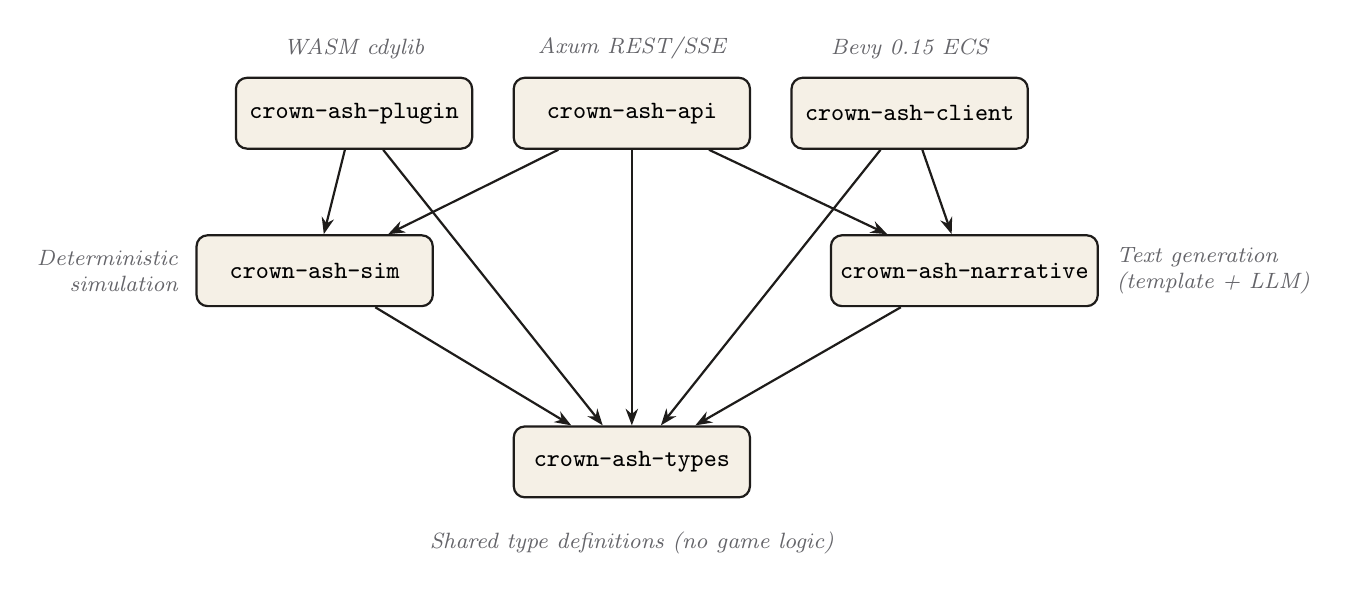
\begin{tikzpicture}[
  crate/.style={draw=cashdark, fill=cashparchment, rounded corners=4pt,
                minimum width=3cm, minimum height=0.9cm, font=\small\ttfamily,
                line width=0.8pt},
  dep/.style={-{Stealth[length=6pt]}, thick, cashdark},
  node distance=1.2cm and 2.5cm,
]
  % Nodes
  \node[crate] (types) {crown-ash-types};
  \node[crate, above left=1.5cm and 1cm of types] (sim) {crown-ash-sim};
  \node[crate, above right=1.5cm and 1cm of types] (narrative) {crown-ash-narrative};
  \node[crate, above=3.5cm of types] (api) {crown-ash-api};
  \node[crate, left=0.5cm of api] (plugin) {crown-ash-plugin};
  \node[crate, right=0.5cm of api] (client) {crown-ash-client};

  % Edges
  \draw[dep] (sim) -- (types);
  \draw[dep] (narrative) -- (types);
  \draw[dep] (api) -- (sim);
  \draw[dep] (api) -- (narrative);
  \draw[dep] (api) -- (types);
  \draw[dep] (plugin) -- (sim);
  \draw[dep] (plugin) -- (types);
  \draw[dep] (client) -- (types);
  \draw[dep] (client) -- (narrative);

  % Labels
  \node[below=0.3cm of types, font=\footnotesize\itshape, cashiron]
    {Shared type definitions (no game logic)};
  \node[left=0.1cm of sim, font=\footnotesize\itshape, cashiron, align=right]
    {Deterministic\\simulation};
  \node[right=0.1cm of narrative, font=\footnotesize\itshape, cashiron, align=left]
    {Text generation\\(template + LLM)};
  \node[above=0.1cm of plugin, font=\footnotesize\itshape, cashiron]
    {WASM cdylib};
  \node[above=0.1cm of api, font=\footnotesize\itshape, cashiron]
    {Axum REST/SSE};
  \node[above=0.1cm of client, font=\footnotesize\itshape, cashiron]
    {Bevy 0.15 ECS};
\end{tikzpicture}
\caption{Crown \& Ash crate dependency graph. Arrows point from dependent to dependency.}
\label{fig:crate-deps}
\end{figure}

\begin{table}[htbp]
\centering
\caption{Crate responsibilities.}
\label{tab:crates}
\begin{tabular}{@{}llp{7cm}@{}}
\toprule
\textbf{Crate} & \textbf{Type} & \textbf{Purpose} \\
\midrule
\crateref{types}     & lib   & Shared types: \fp{}, provinces, factions, characters, actions, events, world state. No game logic. \\
\crateref{sim}       & lib   & Deterministic simulation engine: tick pipeline, combat, economy, cohesion, intrigue, diplomacy, religion, trade, map, world generation. \\
\crateref{narrative} & lib   & 4-tier narrative cascade: template prose, personality archetypes, LLM prompt generation. \\
\crateref{api}       & lib   & Axum HTTP handlers: REST endpoints, SSE event streaming, game state management. \\
\crateref{plugin}    & cdylib & WASM plugin: \texttt{on\_init}, \texttt{on\_tick}, \texttt{process\_action}, \texttt{query\_state}. Compiled to \texttt{.wasm} for on-chain execution. \\
\crateref{client}    & bin   & Bevy 0.15 game client: hex map rendering, egui UI panels, SSE networking. Excluded from workspace (bevy\_egui conflicts). \\
\bottomrule
\end{tabular}
\end{table}

\subsection{WASM Plugin Interface}
\label{sec:wasm}

The simulation is compiled as a \texttt{cdylib} WASM module loaded by the
Q-NarwhalKnight VM. The host--guest interface uses a simple pointer-passing ABI.

\subsubsection{Function ABI}

Every entry point follows the same C-ABI convention:

\begin{lstlisting}[caption={WASM entry point signature.}]
extern "C" fn entry(
    input_ptr: u32,   // pointer to JSON input
    input_len: u32,   // byte length of input
    out_len_ptr: u32, // write output length here
) -> u32              // pointer to JSON output
\end{lstlisting}

The host serializes input as JSON into the guest's linear memory via a bump
allocator starting at offset 65536 (above the WASM stack). The guest
deserializes, executes, serializes the response, and returns a pointer to it.

\subsubsection{Entry Points}

\begin{table}[htbp]
\centering
\caption{WASM plugin entry points.}
\label{tab:entry-points}
\begin{tabular}{@{}llll@{}}
\toprule
\textbf{Entry Point} & \textbf{Input} & \textbf{Output} & \textbf{Purpose} \\
\midrule
\texttt{on\_init}        & \texttt{InitRequest}   & \texttt{InitResponse}   & Create world from config + seed \\
\texttt{on\_tick}         & \texttt{TickRequest}    & \texttt{TickResponse}    & Advance one game turn \\
\texttt{process\_action}  & \texttt{ActionRequest}  & \texttt{ActionResponse}  & Execute a player action \\
\texttt{query\_state}     & \texttt{QueryRequest}   & \texttt{QueryResponse}   & Read-only state query \\
\bottomrule
\end{tabular}
\end{table}

\subsubsection{Host Functions}

The WASM guest imports 9 host functions for storage, events, and utilities:

\begin{table}[htbp]
\centering
\caption{Host functions imported by the WASM plugin.}
\label{tab:host-fns}
\begin{tabular}{@{}lp{8cm}@{}}
\toprule
\textbf{Host Function} & \textbf{Purpose} \\
\midrule
\texttt{plugin\_storage\_read}   & Read a value from persistent plugin storage \\
\texttt{plugin\_storage\_write}  & Write a value to persistent plugin storage \\
\texttt{plugin\_storage\_delete} & Delete a key from plugin storage \\
\texttt{plugin\_storage\_exists} & Check if a key exists \\
\texttt{plugin\_emit\_event}     & Emit a typed blockchain event (topic + data) \\
\texttt{plugin\_get\_block\_height} & Current block height (\texttt{u64}) \\
\texttt{plugin\_get\_timestamp}  & Current UNIX timestamp (\texttt{u64}) \\
\texttt{plugin\_sha3\_256}       & Compute SHA3-256 hash of arbitrary data \\
\texttt{plugin\_log}             & Log message at levels 0 (trace) through 4 (error) \\
\bottomrule
\end{tabular}
\end{table}

\subsection{REST \& SSE API}

The \crateref{api} crate exposes game state through Axum HTTP handlers:

\begin{table}[htbp]
\centering
\caption{Crown \& Ash REST API endpoints.}
\label{tab:api}
\begin{tabular}{@{}llp{6cm}@{}}
\toprule
\textbf{Method} & \textbf{Path} & \textbf{Description} \\
\midrule
\texttt{GET}  & \texttt{/world}           & Full world state snapshot \\
\texttt{GET}  & \texttt{/province/:id}    & Single province details \\
\texttt{GET}  & \texttt{/character/:id}   & Single character details \\
\texttt{GET}  & \texttt{/faction/:id}     & Faction details + relations \\
\texttt{POST} & \texttt{/action}          & Queue a signed player action \\
\texttt{POST} & \texttt{/join}            & Player joins a game session \\
\bottomrule
\end{tabular}
\end{table}

Real-time updates are delivered via Server-Sent Events (SSE) on the main
Q-NarwhalKnight SSE stream. Four event types carry narrative content:

\begin{itemize}
  \item \texttt{crown\_ash\_event} --- Tier 0 structured JSON data
  \item \texttt{crown\_ash\_prose} --- Tier 1 template-generated text
  \item \texttt{crown\_ash\_dialog} --- Tier 2 LLM-generated character dialog
  \item \texttt{crown\_ash\_epic} --- Tier 3 deep LLM narrative
\end{itemize}


% ══════════════════════════════════════════════════════════════════
\section{Deterministic Foundations}
\label{sec:determinism}
% ══════════════════════════════════════════════════════════════════

Every node in the Q-NarwhalKnight network must compute identical game states.
This section describes the two mechanisms that guarantee determinism:
fixed-point arithmetic and a seeded pseudo-random number generator.

\subsection{Fixed-Point Arithmetic}
\label{sec:fixedpoint}

Crown \& Ash bans IEEE 754 floating-point entirely. All numeric computation
uses a custom \fp{} type:

\begin{lstlisting}[caption={FixedPoint core definition.}]
pub struct FixedPoint(pub i64);

const SCALE: i64 = 1000; // 3 decimal places

impl FixedPoint {
    pub fn from_int(n: i64) -> Self { Self(n * SCALE) }
    pub fn from_fraction(num: i64, den: i64) -> Self {
        Self(num * SCALE / den)
    }
    pub fn mul_fp(self, rhs: Self) -> Self {
        Self(self.0 * rhs.0 / SCALE)
    }
    pub fn checked_div_fp(self, rhs: Self) -> Option<Self> {
        if rhs.0 == 0 { None }
        else { Some(Self(self.0 * SCALE / rhs.0)) }
    }
}
\end{lstlisting}

\textbf{Key properties:}

\begin{itemize}
  \item \textbf{Scale factor}: $1000\times$ ($10^3$). The value
    \texttt{FixedPoint(2750)} represents $2.750$.
  \item \textbf{Range}: $[-9.22 \times 10^{15},\; 9.22 \times 10^{15}]$,
    sufficient for all game quantities.
  \item \textbf{Overflow safety}: Multiplication uses \texttt{i64} intermediate
    products. For the value ranges in Crown \& Ash (populations $\leq 10^5$,
    gold $\leq 10^6$), overflow is impossible.
  \item \textbf{Division by zero}: \texttt{checked\_div\_fp} returns
    \texttt{None}; \texttt{saturating\_div\_fp} returns \texttt{ZERO}.
  \item \textbf{Linear interpolation}: \texttt{lerp(other, t)} where
    $t \in [0, 1000]$ blends between two values without floating-point.
\end{itemize}

\subsection{Deterministic Random Number Generator}
\label{sec:rng}

Randomness is derived exclusively from block hashes using an ARX
(add-rotate-xor) hash mixer:

\begin{lstlisting}[caption={Deterministic RNG construction.}]
pub struct DeterministicRng {
    state: [u8; 32],
}

impl DeterministicRng {
    pub fn new(block_hash: [u8; 32], domain: &str) -> Self {
        // state = hash(block_hash || domain || "CROWN_ASH")
        let mut hasher = ArxHash::new();
        hasher.update(&block_hash);
        hasher.update(domain.as_bytes());
        hasher.update(b"CROWN_ASH");
        Self { state: hasher.finalize() }
    }
}
\end{lstlisting}

\textbf{Domain separation} ensures that different subsystems (combat, economy,
events) receive independent pseudo-random sequences from the same block hash.
For example, \texttt{DeterministicRng::new(hash, "combat")} and
\texttt{DeterministicRng::new(hash, "economy")} produce unrelated streams.

The ARX mixing function applies 16 rounds of add-rotate-xor over 8 state
words initialized from the NIST $\pi$ fractional digits. This is a
non-cryptographic hash optimized for speed and avalanche properties, not
collision resistance.

\textbf{Output methods:}

\begin{itemize}
  \item \texttt{next\_u32()} --- Extract 4 bytes from state as little-endian \texttt{u32}, then re-hash.
  \item \texttt{range(min, max)} --- Uniform \texttt{i64} in $[\text{min}, \text{max})$.
  \item \texttt{chance(num, den)} --- Returns \texttt{true} with probability $\frac{\text{num}}{\text{den}}$.
\end{itemize}

\subsection{Determinism Proof Sketch}

\begin{enumerate}
  \item \textbf{Inputs are deterministic.} Block hashes are consensus-agreed.
    Player actions are signed transactions ordered by DAG-Knight consensus.
  \item \textbf{Arithmetic is deterministic.} \fp{} uses only \texttt{i64}
    operations with defined overflow semantics.
  \item \textbf{RNG is deterministic.} Same block hash + same domain
    $\Rightarrow$ same sequence.
  \item \textbf{Iteration order is deterministic.} All collections are
    \texttt{Vec} (ordered) or sorted by key before iteration. No
    \texttt{HashMap} iteration in game logic.
  \item \textbf{No external I/O.} The WASM sandbox prohibits file, network,
    and clock access. \texttt{plugin\_get\_timestamp} returns the
    consensus-agreed block timestamp.
\end{enumerate}

Therefore, for any block sequence $B_1, B_2, \ldots, B_n$, all nodes compute
identical game states $S_0 \xrightarrow{B_1} S_1 \xrightarrow{B_2} S_2
\cdots \xrightarrow{B_n} S_n$.


% ══════════════════════════════════════════════════════════════════
\section{Campaign Map}
\label{sec:map}
% ══════════════════════════════════════════════════════════════════

The campaign map consists of 25 provinces organized into 7 regional clusters,
each initially controlled by one faction. Province adjacency forms a connected
graph with approximately 63 undirected edges.

\subsection{Province Map}

\begin{figure}[htbp]
\centering
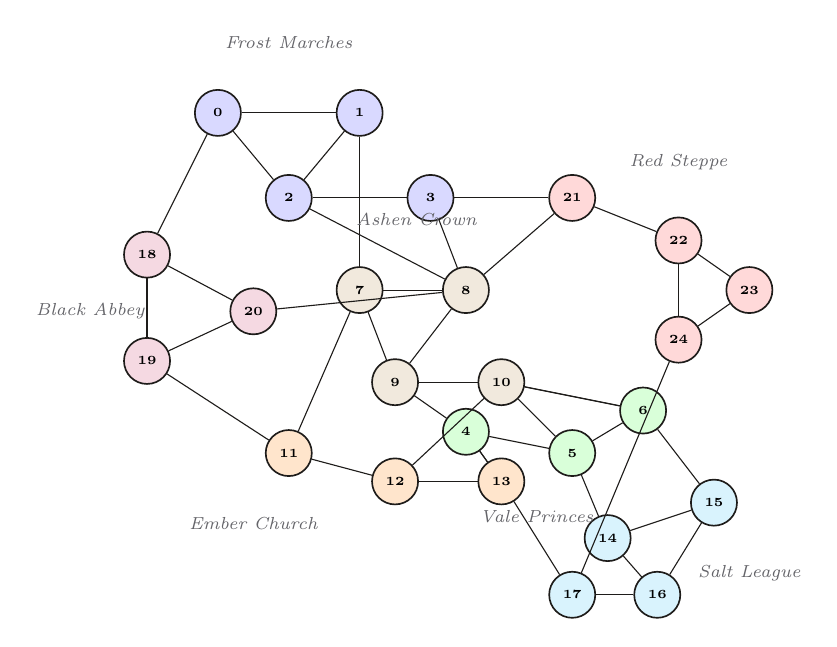
\begin{tikzpicture}[
  prov/.style={circle, draw=cashdark, line width=0.6pt, minimum size=0.65cm,
               font=\tiny\bfseries, inner sep=1pt},
  edge/.style={cashdark, line width=0.4pt},
  label/.style={font=\scriptsize\itshape, cashiron},
  scale=0.9, transform shape,
]
  % ── Frost Marches (blue) ──
  \node[prov, fill=blue!15] (p0) at (0, 6) {0};
  \node[prov, fill=blue!15] (p1) at (2, 6) {1};
  \node[prov, fill=blue!15] (p2) at (1, 4.8) {2};
  \node[prov, fill=blue!15] (p3) at (3, 4.8) {3};

  % ── Black Abbey (purple) ──
  \node[prov, fill=purple!15] (p18) at (-1, 4) {18};
  \node[prov, fill=purple!15] (p19) at (-1, 2.5) {19};
  \node[prov, fill=purple!15] (p20) at (0.5, 3.2) {20};

  % ── Ashen Crown (gray/gold) ──
  \node[prov, fill=cashgold!30] (p7) at (2, 3.5) {7};
  \node[prov, fill=cashgold!30] (p8) at (3.5, 3.5) {8};
  \node[prov, fill=cashgold!30] (p9) at (2.5, 2.2) {9};
  \node[prov, fill=cashgold!30] (p10) at (4, 2.2) {10};

  % ── Red Steppe (red) ──
  \node[prov, fill=red!15] (p21) at (5, 4.8) {21};
  \node[prov, fill=red!15] (p22) at (6.5, 4.2) {22};
  \node[prov, fill=red!15] (p23) at (7.5, 3.5) {23};
  \node[prov, fill=red!15] (p24) at (6.5, 2.8) {24};

  % ── Ember Church (orange) ──
  \node[prov, fill=orange!20] (p11) at (1, 1.2) {11};
  \node[prov, fill=orange!20] (p12) at (2.5, 0.8) {12};
  \node[prov, fill=orange!20] (p13) at (4, 0.8) {13};

  % ── Vale Princes (green) ──
  \node[prov, fill=green!15] (p4) at (3.5, 1.5) {4};
  \node[prov, fill=green!15] (p5) at (5, 1.2) {5};
  \node[prov, fill=green!15] (p6) at (6, 1.8) {6};

  % ── Salt League (cyan) ──
  \node[prov, fill=cyan!15] (p14) at (5.5, 0) {14};
  \node[prov, fill=cyan!15] (p15) at (7, 0.5) {15};
  \node[prov, fill=cyan!15] (p16) at (6.2, -0.8) {16};
  \node[prov, fill=cyan!15] (p17) at (5, -0.8) {17};

  % ── Adjacency edges ──
  \foreach \a/\b in {0/1,0/2,0/18,1/2,1/7,2/3,2/8,3/8,3/21,7/8,7/9,7/11,8/9,8/20,8/21,9/10,9/4,10/5,10/6,10/12,4/5,4/13,5/6,5/14,6/15,6/10,11/12,11/19,12/13,13/4,13/17,14/15,14/16,15/16,16/17,17/24,18/19,18/20,19/20,21/22,22/23,22/24,23/24} {
    \draw[edge] (p\a) -- (p\b);
  }

  % ── Faction labels ──
  \node[label] at (1, 7) {Frost Marches};
  \node[label] at (-1.8, 3.2) {Black Abbey};
  \node[label] at (2.8, 4.5) {Ashen Crown};
  \node[label] at (6.5, 5.3) {Red Steppe};
  \node[label] at (0.5, 0.2) {Ember Church};
  \node[label] at (4.5, 0.3) {Vale Princes};
  \node[label] at (7.5, -0.5) {Salt League};
\end{tikzpicture}
\caption{Campaign map: 25 provinces across 7 factions. Numbers are province IDs;
  colors indicate starting controller.}
\label{fig:map}
\end{figure}

\subsection{Terrain Types}

Each province has an assigned terrain type that affects movement cost and
defensive bonuses in combat.

\begin{table}[htbp]
\centering
\caption{Terrain types with movement costs and defense bonuses.}
\label{tab:terrain}
\begin{tabular}{@{}lcc@{}}
\toprule
\textbf{Terrain} & \textbf{Movement Cost} & \textbf{Defense Bonus} \\
\midrule
Plains    & 1.000 & $+0\%$  \\
Hills     & 1.500 & $+20\%$ \\
Mountains & 2.000 & $+40\%$ \\
Forest    & 1.300 & $+25\%$ \\
Marsh     & 1.800 & $+30\%$ \\
Desert    & 1.400 & $+10\%$ \\
Coastal   & 1.000 & $+15\%$ \\
River     & 1.200 & $+20\%$ \\
\bottomrule
\end{tabular}
\end{table}

\subsection{Improvements}

Players can construct improvements in their provinces. Each has a gold cost,
build time (in turns), and economic or military output.

\begin{table}[htbp]
\centering
\caption{Province improvements.}
\label{tab:improvements}
\begin{tabular}{@{}lccl@{}}
\toprule
\textbf{Improvement} & \textbf{Cost} & \textbf{Turns} & \textbf{Effect} \\
\midrule
Farmstead       & 50  & 3  & +10 food/turn \\
Mine            & 80  & 5  & +5 iron, +3 gold/turn \\
Lumbercamp      & 40  & 3  & +8 timber/turn \\
Quarry          & 60  & 5  & +6 stone/turn \\
Stables         & 70  & 5  & +5 horses/turn \\
Market          & 100 & 7  & +2.000 prosperity, +gold \\
Temple          & 120 & 7  & +clerical favor \\
Fortification   & 150 & 12 & +defense level (+10\%/level) \\
University      & 200 & 10 & +learning bonus \\
Port (coastal)  & 130 & 10 & +trade capacity \\
Granary         & 45  & 3  & Famine resistance \\
Hospital        & 90  & 7  & Plague resistance \\
\bottomrule
\end{tabular}
\end{table}

\subsection{Pathfinding}

Province connectivity is stored as an adjacency list. Pathfinding uses
breadth-first search, which is optimal for unweighted graphs and trivially
bounded: $O(V + E) = O(25 + 63) = O(88)$.

\begin{lstlisting}[caption={BFS pathfinding API.}]
pub fn find_path(start: u16, goal: u16) -> Option<Vec<u16>>;
pub fn path_length(start: u16, goal: u16) -> Option<usize>;
\end{lstlisting}


% ══════════════════════════════════════════════════════════════════
\section{The Seven Factions}
\label{sec:factions}
% ══════════════════════════════════════════════════════════════════

Each faction has a unique culture, religion, starting provinces, and a set of
\fp{} multipliers that scale military, economic, diplomatic, and religious
effectiveness.

\begin{table}[htbp]
\centering
\caption{Faction bonuses and characteristics.}
\label{tab:factions}
\small
\begin{tabular}{@{}clllcccc@{}}
\toprule
\textbf{ID} & \textbf{Name} & \textbf{Culture} & \textbf{Religion} &
  \textbf{Mil.} & \textbf{Econ.} & \textbf{Dipl.} & \textbf{Decay} \\
\midrule
0 & Ashen Crown   & Imperial   & Ember Church  & 0.900 & 1.000 & 1.200 & 0.900 \\
1 & Vale Princes  & Feudal     & Ember Church  & 1.100 & 1.300 & 1.000 & 1.200 \\
2 & Ember Church  & Clerical   & Ember Church  & 0.800 & 1.000 & 1.000 & 0.800 \\
3 & Salt League   & Mercantile & Salt Cult     & 1.000 & 1.500 & 1.200 & 1.100 \\
4 & Frost Marches & Nordic     & Frost Spirits & 1.400 & 1.000 & 0.800 & 1.000 \\
5 & Red Steppe    & Nomadic    & Old Faith     & 1.300 & 0.600 & 1.000 & 1.300 \\
6 & Black Abbey   & Monastic   & Black Order   & 1.000 & 1.000 & 0.800 & 1.000 \\
\bottomrule
\end{tabular}
\end{table}

\textbf{Decay} is the cohesion decay rate multiplier ($\S$\ref{sec:cohesion}).
A value below 1.000 means the faction's realm stability decays slower than
baseline (institutional advantage); above 1.000 means faster decay (nomadic
instability).

\subsection{Dynasties and Succession}

Each faction's ruling dynasty is tracked through a full character graph
including marriages, children, and inheritance claims. When a ruler dies,
succession follows these rules:

\begin{enumerate}
  \item \textbf{Designated heir}: If the ruler used \texttt{DesignateHeir},
    that character inherits.
  \item \textbf{Eldest child}: The oldest living child of the same dynasty.
  \item \textbf{Dynasty member}: Any living character of the same dynasty.
  \item \textbf{Succession crisis}: If no valid heir exists, the realm may
    fracture---triggering a \texttt{RealmSplit} event.
\end{enumerate}

A succession crisis can cause provinces to defect to a rebel faction led by
the strongest rival claimant, reducing the original realm's territory.


% ══════════════════════════════════════════════════════════════════
\section{Simulation Engine}
\label{sec:sim}
% ══════════════════════════════════════════════════════════════════

The simulation engine (\crateref{sim}) is the heart of Crown \& Ash. It
processes one game turn per invocation of \texttt{tick()}, which is called
every \texttt{BLOCKS\_PER\_TURN = 10} blockchain blocks.

\subsection{Tick Pipeline}

Figure~\ref{fig:pipeline} shows the 10+ phase pipeline executed each turn.

\begin{figure}[htbp]
\centering
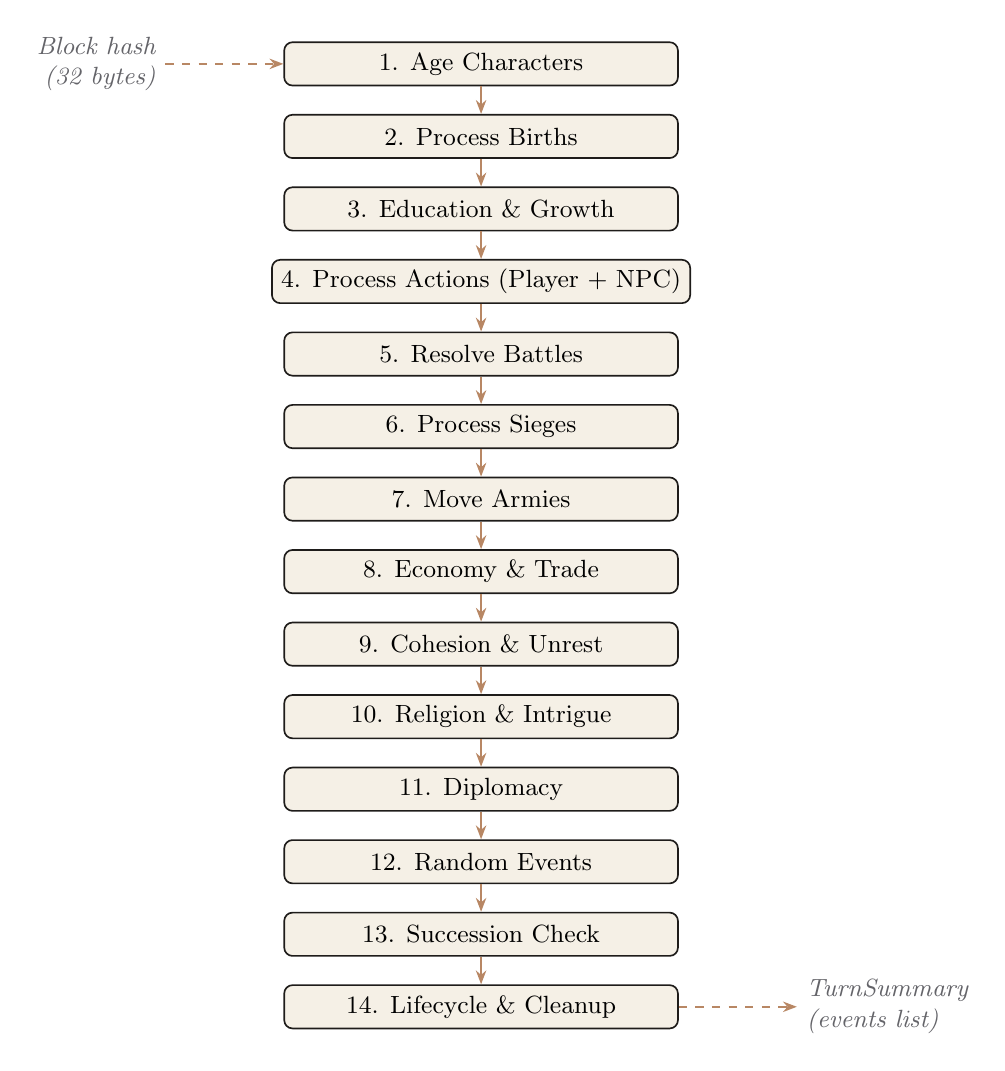
\begin{tikzpicture}[
  phase/.style={draw=cashdark, fill=cashparchment, rounded corners=3pt,
                minimum width=5cm, minimum height=0.55cm,
                font=\small, line width=0.6pt},
  arr/.style={-{Stealth[length=5pt]}, cashcopper, thick},
  node distance=0.35cm,
]
  \node[phase] (p1) {1. Age Characters};
  \node[phase, below=of p1] (p2) {2. Process Births};
  \node[phase, below=of p2] (p3) {3. Education \& Growth};
  \node[phase, below=of p3] (p4) {4. Process Actions (Player + NPC)};
  \node[phase, below=of p4] (p5) {5. Resolve Battles};
  \node[phase, below=of p5] (p6) {6. Process Sieges};
  \node[phase, below=of p6] (p7) {7. Move Armies};
  \node[phase, below=of p7] (p8) {8. Economy \& Trade};
  \node[phase, below=of p8] (p9) {9. Cohesion \& Unrest};
  \node[phase, below=of p9] (p10) {10. Religion \& Intrigue};
  \node[phase, below=of p10] (p11) {11. Diplomacy};
  \node[phase, below=of p11] (p12) {12. Random Events};
  \node[phase, below=of p12] (p13) {13. Succession Check};
  \node[phase, below=of p13] (p14) {14. Lifecycle \& Cleanup};

  \foreach \a/\b in {p1/p2, p2/p3, p3/p4, p4/p5, p5/p6, p6/p7, p7/p8,
                     p8/p9, p9/p10, p10/p11, p11/p12, p12/p13, p13/p14} {
    \draw[arr] (\a) -- (\b);
  }

  % Block hash input
  \node[left=1.5cm of p1, font=\small\itshape, cashiron, align=right]
    (seed) {Block hash\\(32 bytes)};
  \draw[arr, dashed] (seed) -- (p1);

  % Output
  \node[right=1.5cm of p14, font=\small\itshape, cashiron, align=left]
    (out) {TurnSummary\\(events list)};
  \draw[arr, dashed] (p14) -- (out);
\end{tikzpicture}
\caption{Tick pipeline: 14 phases per game turn, seeded by the block hash.}
\label{fig:pipeline}
\end{figure}

\begin{algorithm}[htbp]
\caption{Tick Pipeline (simplified)}
\label{alg:tick}
\begin{algorithmic}[1]
\Require $\mathit{world}$: mutable GameWorld, $\mathit{hash}$: 32-byte block hash
\Ensure $\mathit{summary}$: TurnSummary (list of events)
\State $\mathit{rng} \gets \textsc{DeterministicRng}(\mathit{hash})$
\State $\mathit{events} \gets []$
\State \textsc{AgeCharacters}($\mathit{world}$, $\mathit{rng}$, $\mathit{events}$) \Comment{natural death}
\State \textsc{ProcessBirths}($\mathit{world}$, $\mathit{rng}$, $\mathit{events}$) \Comment{cap: 5/turn}
\State \textsc{Education}($\mathit{world}$, $\mathit{rng}$)
\State \textsc{ProcessActions}($\mathit{world}$, $\mathit{rng}$, $\mathit{events}$) \Comment{player + NPC AI}
\State \textsc{ResolveBattles}($\mathit{world}$, $\mathit{rng}$, $\mathit{events}$) \Comment{cap: 5/turn}
\State \textsc{ProcessSieges}($\mathit{world}$, $\mathit{rng}$, $\mathit{events}$)
\State \textsc{MoveArmies}($\mathit{world}$)
\State \textsc{Economy}($\mathit{world}$, $\mathit{events}$)
\State \textsc{Trade}($\mathit{world}$, $\mathit{events}$)
\State \textsc{Cohesion}($\mathit{world}$) ; \textsc{Unrest}($\mathit{world}$)
\State \textsc{Religion}($\mathit{world}$, $\mathit{rng}$, $\mathit{events}$)
\State \textsc{Intrigue}($\mathit{world}$, $\mathit{rng}$, $\mathit{events}$) \Comment{cap: 20 plots}
\State \textsc{Diplomacy}($\mathit{world}$, $\mathit{events}$)
\State \textsc{RandomEvents}($\mathit{world}$, $\mathit{rng}$, $\mathit{events}$) \Comment{cap: 10/turn}
\State \textsc{SuccessionCheck}($\mathit{world}$, $\mathit{rng}$, $\mathit{events}$) \Comment{cap: 3/turn}
\State \textsc{Lifecycle}($\mathit{world}$) \Comment{tombstone dead, enforce caps}
\State \Return $\textsc{TurnSummary}(\mathit{events})$
\end{algorithmic}
\end{algorithm}

\subsection{Combat System}
\label{sec:combat}

Battles are resolved automatically when opposing armies occupy the same province.

\subsubsection{Power Calculation}

\begin{figure}[htbp]
\centering
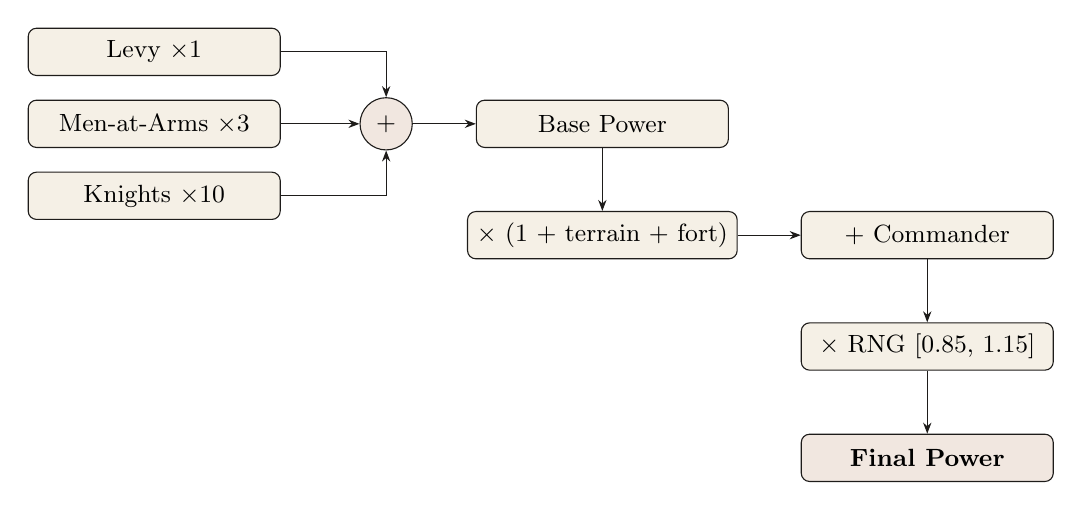
\begin{tikzpicture}[
  box/.style={draw=cashdark, fill=cashparchment, rounded corners=3pt,
              minimum width=3.2cm, minimum height=0.6cm, font=\small},
  op/.style={circle, draw=cashdark, fill=cashcopper!20, minimum size=0.5cm,
             font=\small\bfseries},
  arr/.style={-{Stealth[length=4pt]}, cashdark},
  node distance=0.8cm,
]
  \node[box] (levy) {Levy $\times 1$};
  \node[box, below=0.3cm of levy] (maa) {Men-at-Arms $\times 3$};
  \node[box, below=0.3cm of maa] (kn) {Knights $\times 10$};
  \node[op, right=1cm of maa] (plus1) {$+$};
  \draw[arr] (levy) -| (plus1);
  \draw[arr] (maa) -- (plus1);
  \draw[arr] (kn) -| (plus1);

  \node[box, right=0.8cm of plus1] (base) {Base Power};
  \draw[arr] (plus1) -- (base);

  \node[box, below=0.8cm of base] (terrain) {$\times$ (1 + terrain + fort)};
  \draw[arr] (base) -- (terrain);

  \node[box, right=0.8cm of terrain] (cmd) {$+$ Commander};
  \draw[arr] (terrain) -- (cmd);

  \node[box, below=0.8cm of cmd] (rng) {$\times$ RNG [0.85, 1.15]};
  \draw[arr] (cmd) -- (rng);

  \node[box, below=0.8cm of rng, fill=cashcopper!20] (final) {\textbf{Final Power}};
  \draw[arr] (rng) -- (final);
\end{tikzpicture}
\caption{Combat power calculation flow.}
\label{fig:combat}
\end{figure}

The combat formula in \fp{} arithmetic:

\begin{align}
  \text{attack} &= \text{levy} \times 1 + \text{men\_at\_arms} \times 3 + \text{knights} \times 10 \\
  \text{defense} &= \text{attack} \times \frac{1000 + \text{terrain\_bonus} + \text{fort\_bonus}}{1000} \\
  \text{cmd\_bonus} &= \text{martial\_stat} \times 10 \\
  \text{rng\_factor} &\sim \text{Uniform}[850, 1150] \\
  \text{final} &= (\text{power} + \text{cmd\_bonus}) \times \frac{\text{rng\_factor}}{1000}
\end{align}

\subsubsection{Casualty Resolution}

\begin{itemize}
  \item \textbf{Winner casualties}: 20--30\% of engaged troops (base 200--300).
  \item \textbf{Loser casualties}: 40--60\% of engaged troops (base 400--600).
  \item \textbf{Morale collapse}: If casualties exceed 40\% of the original
    army size, morale drops to 100 (minimum), preventing further offensive
    action until reinforced.
  \item \textbf{Retreat}: The losing army retreats to a random adjacent
    province controlled by their faction. Armies with no valid retreat
    destination are destroyed.
\end{itemize}

\subsubsection{Siege Mechanics}

Sieges occur when an army attacks a fortified province. Unlike field battles,
sieges resolve over multiple turns:

\begin{itemize}
  \item \textbf{Duration}: Proportional to fortification level (base 3 turns + 2/level).
  \item \textbf{Attrition}: Besieging army takes casualties each turn.
  \item \textbf{Completion}: Province control transfers on siege completion.
\end{itemize}

\subsection{Economy}
\label{sec:economy}

\subsubsection{Tax Collection}

Each turn, provinces generate tax revenue:

\begin{equation}
  \text{tax\_gold} = \frac{\text{population} \times \text{tax\_rate} \times \text{prosperity}}{1{,}000{,}000}
\end{equation}

where all values are \fp{} (scale 1000). Tax rate is player-configurable
from 0 to 1000 (0\% to 100\%).

\subsubsection{Prosperity Dynamics}

Prosperity is the primary economic health indicator, ranging from 50.000
(destitute) to 1000.000 (flourishing):

\begin{table}[htbp]
\centering
\caption{Prosperity modifiers per turn.}
\label{tab:prosperity}
\begin{tabular}{@{}lrl@{}}
\toprule
\textbf{Condition} & \textbf{Change} & \textbf{Notes} \\
\midrule
Peace (no war, unrest $\leq$ 500) & $+2.000$ & Baseline growth \\
Active war                        & $-5.000$ & Faction at war \\
Farmstead improvement             & $+1.000$ & Per turn bonus \\
Market improvement                & $+2.000$ & Per turn bonus \\
\bottomrule
\end{tabular}
\end{table}

\subsubsection{Population Growth}

\begin{itemize}
  \item \textbf{Growth}: If prosperity $> 500$, population grows by $+0.1\%$ per turn.
  \item \textbf{Decline}: If prosperity $< 200$, population declines by $-0.2\%$ per turn.
  \item \textbf{Floor}: No province drops below 100 population.
\end{itemize}

\subsection{Realm Cohesion}
\label{sec:cohesion}

Realm stability is modeled through five independent cohesion components, each
ranging from 0 to 1000:

\begin{table}[htbp]
\centering
\caption{Cohesion components.}
\label{tab:cohesion}
\begin{tabular}{@{}lp{8cm}@{}}
\toprule
\textbf{Component} & \textbf{Description} \\
\midrule
Legitimacy         & The ruler's perceived right to rule. Boosted by high martial stat. \\
Fealty             & Vassal loyalty. Boosted by high diplomacy. \\
Clerical Favor     & Church/religious institution support. Boosted by high learning. \\
Commoner Mood      & General population happiness. Reduced by war, boosted by stewardship. \\
Regional Identity  & Cultural unity. Drops sharply ($-30$) when a province is conquered. \\
\bottomrule
\end{tabular}
\end{table}

Each component decays toward equilibrium (500) at a base rate of $0.010$/turn,
modified by the faction's decay multiplier. If \emph{any} component drops
below 200, the realm risks fracture: provinces may rebel, triggering a
\texttt{RealmSplit} event.

\subsection{Intrigue}
\label{sec:intrigue}

The intrigue system models espionage through four plot types:

\begin{table}[htbp]
\centering
\caption{Intrigue plot types and effects.}
\label{tab:plots}
\begin{tabular}{@{}llrl@{}}
\toprule
\textbf{Plot Type} & \textbf{Effect} & \textbf{Fire Threshold} & \textbf{Notes} \\
\midrule
Assassination & Kill target character     & 1000 & 70\% base success \\
Fabricate     & Create province claim     & 1000 & Enables war \\
Sabotage      & $-200$ prosperity         & 1000 & Economic warfare \\
Steal         & $-100$ gold from treasury & 1000 & Subterfuge \\
\bottomrule
\end{tabular}
\end{table}

\textbf{Plot progress} advances each turn:
\begin{equation}
  \text{progress} = \text{instigator.intrigue} \times 20 + \sum_{\text{backers}} \text{backer.intrigue} \times 5
\end{equation}

Plots fire when progress reaches 1000. \textbf{Counter-intelligence} is handled by
the target's spymaster: if $\text{spymaster.intrigue} \times 10 >
\text{plot.secrecy}$, the plot is discovered. The Paranoid trait grants $+200$
discovery bonus.

\textbf{Work cap}: Maximum 20 active plots globally, 3 executions per turn.


% ══════════════════════════════════════════════════════════════════
\section{NPC AI}
\label{sec:ai}
% ══════════════════════════════════════════════════════════════════

Non-player factions are controlled by a heuristic decision framework that
runs during phase 4 (Process Actions) of each tick. The AI evaluates the
faction's current state and selects actions from the same
\texttt{GameAction} enum available to human players.

\subsection{Decision Priorities}

The AI evaluates actions in priority order:

\begin{enumerate}
  \item \textbf{Survival}: If any cohesion component $< 250$, prioritize
    stabilization (lower taxes, appease clergy, assign steward).
  \item \textbf{Military threat}: If enemy armies are in controlled provinces,
    raise armies and engage.
  \item \textbf{Expansion}: If military strength exceeds neighbors by $> 50\%$
    and legitimacy $> 600$, consider declaring war.
  \item \textbf{Economy}: Build improvements in provinces with the highest
    ROI (markets in high-population provinces, farmsteads in low-prosperity).
  \item \textbf{Intrigue}: Rulers with the Schemer or Deceitful trait are more
    likely to launch plots against rivals.
  \item \textbf{Diplomacy}: Propose treaties with factions that share a
    religion or have high mutual opinion.
\end{enumerate}

\subsection{Limitations}

The current NPC AI is deliberately simple:

\begin{itemize}
  \item No multi-turn planning or look-ahead.
  \item No coalition formation.
  \item Personality traits influence action \emph{weights} but do not
    fundamentally change the decision tree.
  \item The AI uses the same deterministic RNG as all other systems, ensuring
    reproducibility.
\end{itemize}

\placeholder{Advanced AI behaviors (feudal obligation simulation, bluffing in
diplomacy, strategic retreat) are planned for future versions.}


% ══════════════════════════════════════════════════════════════════
\section{Narrative Engine}
\label{sec:narrative}
% ══════════════════════════════════════════════════════════════════

Crown \& Ash transforms raw game events into prose through a 4-tier narrative
cascade. The system is designed to provide instant feedback for routine events
while reserving expensive LLM generation for dramatic moments.

\subsection{Cascade Architecture}

\begin{figure}[htbp]
\centering
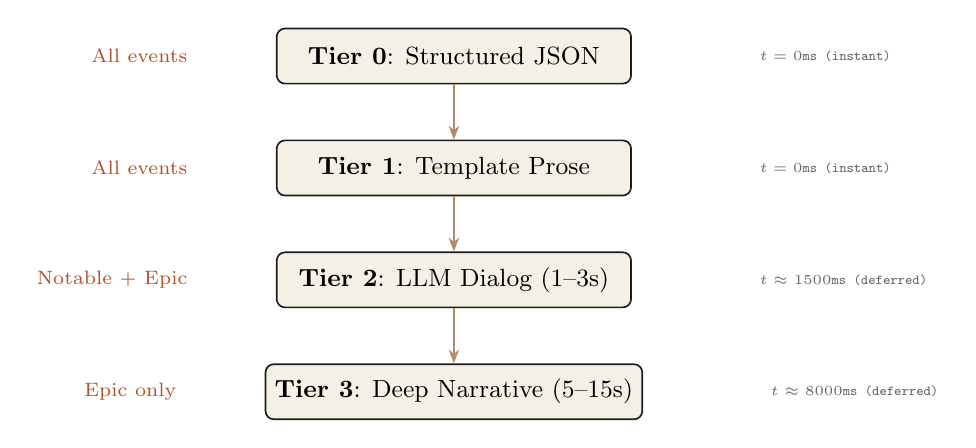
\begin{tikzpicture}[
  tier/.style={draw=cashdark, fill=cashparchment, rounded corners=3pt,
               minimum width=4.5cm, minimum height=0.7cm, font=\small,
               line width=0.6pt},
  time/.style={font=\tiny\ttfamily, cashiron},
  arr/.style={-{Stealth[length=5pt]}, cashcopper, thick},
  node distance=0.7cm,
]
  \node[tier] (t0) {\textbf{Tier 0}: Structured JSON};
  \node[tier, below=of t0] (t1) {\textbf{Tier 1}: Template Prose};
  \node[tier, below=of t1] (t2) {\textbf{Tier 2}: LLM Dialog (1--3s)};
  \node[tier, below=of t2] (t3) {\textbf{Tier 3}: Deep Narrative (5--15s)};

  \draw[arr] (t0) -- (t1);
  \draw[arr] (t1) -- (t2);
  \draw[arr] (t2) -- (t3);

  % Timing
  \node[time, right=1.5cm of t0] {$t = 0\text{ms}$ (instant)};
  \node[time, right=1.5cm of t1] {$t = 0\text{ms}$ (instant)};
  \node[time, right=1.5cm of t2] {$t \approx 1500\text{ms}$ (deferred)};
  \node[time, right=1.5cm of t3] {$t \approx 8000\text{ms}$ (deferred)};

  % Event class labels
  \node[font=\scriptsize, cashember, left=1cm of t0] {All events};
  \node[font=\scriptsize, cashember, left=1cm of t1] {All events};
  \node[font=\scriptsize, cashember, left=1cm of t2] {Notable + Epic};
  \node[font=\scriptsize, cashember, left=1cm of t3] {Epic only};
\end{tikzpicture}
\caption{4-tier narrative cascade. Lower tiers fire only for high-importance events.}
\label{fig:cascade}
\end{figure}

\subsection{Importance Classification}

Events are classified into three importance levels that determine which
narrative tiers activate:

\begin{table}[htbp]
\centering
\caption{Event importance classification.}
\label{tab:importance}
\begin{tabular}{@{}lp{6cm}l@{}}
\toprule
\textbf{Level} & \textbf{Trigger Examples} & \textbf{Tiers} \\
\midrule
\textbf{Minor}    & Harvest, construction complete, routine diplomacy & 0, 1 \\
\textbf{Notable}  & Province conquered, war declared, treaty signed, plot success, rebellion ($>200$ rebels) & 0, 1, 2 \\
\textbf{Epic}     & Faction eliminated, realm split, succession crisis, massive battle ($>500$ casualties) & 0, 1, 2, 3 \\
\bottomrule
\end{tabular}
\end{table}

\subsection{Personality Archetypes}
\label{sec:archetypes}

Character dialog is flavored by personality archetypes derived from trait
combinations. The \crateref{narrative} crate maps each character's traits to
one of 10 archetypes, which provides tone descriptors and speech patterns for
LLM prompting.

\begin{table}[htbp]
\centering
\caption{Personality archetypes and their derivation.}
\label{tab:archetypes}
\small
\begin{tabular}{@{}llp{5.5cm}@{}}
\toprule
\textbf{Archetype} & \textbf{Traits Required} & \textbf{Tone \& Speech} \\
\midrule
Tyrant     & Cruel/Wrathful + Brave       & Menacing, authoritative. ``Obedience or death.'' \\
Saint      & Pious + Kind/Just            & Gentle, compassionate. ``May the gods guide us.'' \\
Schemer    & Schemer / Deceitful+Ambitious & Calculating, smooth. ``Trust is a luxury.'' \\
Commander  & Brave + Just/Strategist      & Decisive, honorable. ``For glory!'' \\
Diplomat   & Gregarious + Kind/Honest     & Warm, persuasive. ``Peace through trade.'' \\
Scholar    & Scholar / Patient+Diligent   & Measured, thoughtful. ``Knowledge is power.'' \\
Conqueror  & Ambitious + Wrathful/Brave   & Bold, commanding. ``Seize destiny!'' \\
Hedonist   & Content + Slothful/Gluttonous & Languid, amused. ``Enjoy the feast.'' \\
Inquisitor & Paranoid + Cruel/Cynical     & Suspicious, sharp. ``Who can be trusted?'' \\
Balanced   & No dominant pattern           & Measured, pragmatic. Neutral tone. \\
\bottomrule
\end{tabular}
\end{table}

\subsection{LLM Generation}

Tier 2 and Tier 3 narratives are generated by passing structured context to
an LLM:

\begin{itemize}
  \item \textbf{Tier 2 (dialog)}: Short character speech (1--3 sentences).
    The prompt includes the character's archetype tone, the event context,
    and faction relationships. Generated asynchronously; delivered via
    \texttt{crown\_ash\_dialog} SSE events.
  \item \textbf{Tier 3 (deep narrative)}: Multi-paragraph dramatic prose
    describing epic events from a narrator's perspective. Only triggered for
    Epic-class events. Delivered via \texttt{crown\_ash\_epic} SSE events.
\end{itemize}

The LLM is accessed through the Q-NarwhalKnight node's inference engine
(when available). If no LLM is available, only Tier 0 and Tier 1 output
is generated---the game remains fully playable without narrative enrichment.


% ══════════════════════════════════════════════════════════════════
\section{Client Architecture}
\label{sec:client}
% ══════════════════════════════════════════════════════════════════

The Crown \& Ash client is built on Bevy 0.15 with an Entity Component System
(ECS) architecture. It is compiled as a standalone binary, separate from the
workspace (due to bevy\_egui dependency conflicts).

\subsection{Plugin Structure}

\begin{table}[htbp]
\centering
\caption{Bevy client plugins.}
\label{tab:plugins}
\begin{tabular}{@{}lp{4cm}p{5cm}@{}}
\toprule
\textbf{Plugin} & \textbf{Systems} & \textbf{Resources} \\
\midrule
\texttt{CrownAshNetworkPlugin} & API polling, SSE listener & API state, SSE stream \\
\texttt{CrownAshMapPlugin}     & Map rendering, terrain display & Map state, province meshes \\
\texttt{CrownAshUiPlugin}      & UI panels, action submission, narrative display & Game state, narrative state, selection state \\
\bottomrule
\end{tabular}
\end{table}

\subsection{ECS Design}

\begin{itemize}
  \item \textbf{Provinces}: One entity per province with terrain mesh
    components, colored by controlling faction.
  \item \textbf{Armies}: Entities with position, troop count, and faction
    marker components.
  \item \textbf{Selection}: A global \texttt{SelectionState} resource tracks
    the currently selected province, army, or character for UI panel display.
  \item \textbf{Narrative}: A \texttt{NarrativeState} resource queues
    incoming SSE events and tier-based narrative text for the event log panel.
\end{itemize}

\subsection{Rendering}

The map is rendered as a 2D hex grid using Bevy's sprite system:

\begin{itemize}
  \item Province territories are colored by faction ownership.
  \item Terrain types use distinct visual patterns.
  \item Armies are represented as shield icons with troop count labels.
  \item UI panels use egui for immediate-mode rendering of faction info,
    province details, character sheets, and the event log.
\end{itemize}

\subsection{Networking}

The client connects to the Q-NarwhalKnight node via:

\begin{enumerate}
  \item \textbf{REST polling}: Fetches the full \texttt{GameWorld} on
    startup and periodically refreshes.
  \item \textbf{SSE streaming}: Subscribes to the node's SSE endpoint for
    real-time \texttt{crown\_ash\_*} events, eliminating the need for
    full-state polling after initial sync.
  \item \textbf{Action submission}: Player actions are POSTed to
    \texttt{/action} as signed JSON payloads.
\end{enumerate}


% ══════════════════════════════════════════════════════════════════
\section{Security}
\label{sec:security}
% ══════════════════════════════════════════════════════════════════

Running a strategy game on a public blockchain introduces unique security
considerations. Crown \& Ash addresses these through multiple layers of
defense.

\subsection{Consensus Safety}

Because the game state is computed deterministically from the block sequence,
consensus safety inherits directly from Q-NarwhalKnight's DAG-BFT protocol:

\begin{itemize}
  \item \textbf{Finality}: Game state changes are final once the
    corresponding blocks achieve DAG-Knight finality ($< 2.9$s).
  \item \textbf{Fork resistance}: If a chain fork occurs, both branches
    produce valid but divergent game states. On fork resolution, the
    losing branch's game state is discarded and recomputed from the
    winning chain.
  \item \textbf{SIM\_VERSION check}: Nodes with mismatched simulation
    versions reject each other's game state, preventing desynchronization.
\end{itemize}

\subsection{Action Validation}

Player actions undergo multi-layer validation:

\begin{enumerate}
  \item \textbf{Signature verification}: Every action is a signed
    transaction. Invalid signatures are rejected before processing.
  \item \textbf{Wallet--faction binding}: A player's wallet is bound to
    exactly one faction at join time. Actions targeting provinces or
    characters outside the player's faction are rejected.
  \item \textbf{Rule validation}: The simulation engine validates action
    legality (e.g., cannot raise armies in uncontrolled provinces, cannot
    declare war on allies, cannot build improvements already under
    construction).
  \item \textbf{Rate limiting}: One action per player per turn, enforced
    at the API layer.
\end{enumerate}

\subsection{Anti-Cheat}

\begin{itemize}
  \item \textbf{No client authority}: The client is a pure display layer.
    All state transitions occur in the WASM sandbox. A modified client
    cannot produce invalid state.
  \item \textbf{Deterministic verification}: Any observer can replay the
    chain and verify every game state transition. Cheating would require
    compromising blockchain consensus itself.
  \item \textbf{No hidden information}: All game state is on-chain and
    visible to all nodes. There is no fog of war in the current version.
    \placeholder{Encrypted state with zero-knowledge proofs for fog-of-war.}
\end{itemize}

\subsection{Work Caps}

To prevent denial-of-service through computationally expensive game states,
every tick phase has hard limits:

\begin{table}[htbp]
\centering
\caption{Per-turn work caps.}
\label{tab:workcaps}
\begin{tabular}{@{}lr@{}}
\toprule
\textbf{Operation} & \textbf{Max per Turn} \\
\midrule
Battles resolved     & 5 \\
Random events        & 10 \\
Births               & 5 \\
Deaths               & 5 \\
Succession checks    & 3 \\
Active plots (global) & 20 \\
Plot executions      & 3 \\
\bottomrule
\end{tabular}
\end{table}

These caps ensure that WASM execution time remains bounded regardless of game
state complexity, preventing a single game from starving the blockchain of
resources.


% ══════════════════════════════════════════════════════════════════
\section{Roadmap}
\label{sec:roadmap}
% ══════════════════════════════════════════════════════════════════

\begin{table}[htbp]
\centering
\caption{Development roadmap. Update the \textbf{Status} column as work progresses.}
\label{tab:roadmap}
\begin{tabular}{@{}clp{5.5cm}l@{}}
\toprule
\textbf{Phase} & \textbf{Name} & \textbf{Features} & \textbf{Status} \\
\midrule
1 & Core Simulation    & Tick pipeline, combat, economy, factions, provinces, map & \textsc{complete} \\
2 & Character Depth    & Traits, dynasties, succession, marriage, education & \textsc{complete} \\
3 & Espionage          & Intrigue plots, counter-intelligence, spymasters & \textsc{complete} \\
4 & Narrative          & 4-tier cascade, personality archetypes, LLM integration & \textsc{complete} \\
5 & Client             & Bevy 0.15 client, hex map, egui panels, SSE networking & \textsc{complete} \\
6 & Diplomacy+         & Advanced treaties, coalition wars, tributary system & \textsc{in progress} \\
7 & Religion+          & Great schisms, heresies, crusade mechanics & \textsc{planned} \\
8 & Fog of War         & ZK-encrypted state, selective revelation & \textsc{planned} \\
9 & Modding            & User-uploadable WASM scenario packs & \textsc{planned} \\
10 & Multiplayer+      & Competitive seasons, ranked matches, spectator mode & \textsc{planned} \\
\bottomrule
\end{tabular}
\end{table}


% ══════════════════════════════════════════════════════════════════
\section{Conclusion}
\label{sec:conclusion}
% ══════════════════════════════════════════════════════════════════

Crown \& Ash demonstrates that complex, deep strategy games can run
\emph{entirely} on a blockchain without sacrificing gameplay depth for
financial mechanics. By compiling the simulation to deterministic WASM,
using fixed-point arithmetic throughout, and seeding randomness from
consensus-agreed block hashes, every node independently computes identical
game states---making the blockchain itself the authoritative game server.

The 6-crate architecture separates concerns cleanly: types define the data
model, the simulation engine processes game logic, the narrative engine adds
literary flavor, the plugin compiles to on-chain WASM, the API exposes state
to clients, and the Bevy client renders it all. This modularity enables
independent development of each layer and straightforward extension as new
game systems (advanced diplomacy, fog of war, modding) are added.

Crown \& Ash is not finished---it is a living system designed for continuous
expansion. The version macros, modular sections, and roadmap table in this
paper are structured for easy updates as the game evolves.


% ══════════════════════════════════════════════════════════════════
\appendix
% ══════════════════════════════════════════════════════════════════

\section{Game Constants Reference}
\label{app:constants}

\begin{longtable}{@{}llrl@{}}
\caption{Complete game constants reference.} \label{tab:constants} \\
\toprule
\textbf{Constant} & \textbf{Module} & \textbf{Value} & \textbf{Description} \\
\midrule
\endfirsthead
\toprule
\textbf{Constant} & \textbf{Module} & \textbf{Value} & \textbf{Description} \\
\midrule
\endhead
\midrule
\multicolumn{4}{r}{\textit{Continued on next page}} \\
\endfoot
\bottomrule
\endlastfoot
\texttt{SIM\_VERSION}             & world    & \simversion & Simulation version string \\
\texttt{BLOCKS\_PER\_TURN}        & world    & 10    & Blocks per game turn \\
\texttt{MAX\_FACTIONS}            & world    & 7     & Maximum factions \\
\texttt{MAX\_PROVINCES}           & world    & 25    & Maximum provinces \\
\texttt{SCALE}                    & fixed\_point & 1000 & FixedPoint scale factor \\
\texttt{MAX\_BATTLES\_PER\_TURN}  & combat   & 5     & Battle resolution cap \\
\texttt{MAX\_EVENTS\_PER\_TURN}   & tick     & 10    & Random event cap \\
\texttt{MAX\_SUCCESSIONS\_PER\_TURN} & tick  & 3     & Succession check cap \\
\texttt{MAX\_BIRTHS\_PER\_TURN}   & tick     & 5     & Birth event cap \\
\texttt{MAX\_DEATHS\_PER\_TURN}   & tick     & 5     & Death event cap \\
\texttt{BASE\_DECAY\_RATE}        & cohesion & 0.010 & Cohesion decay/turn \\
\texttt{WAR\_MOOD\_PENALTY}       & cohesion & $-3.000$ & Commoner mood per turn at war \\
\texttt{CONQUEST\_IDENTITY\_PENALTY} & cohesion & $-30.000$ & One-time identity loss \\
\texttt{FORT\_BONUS\_PER\_LEVEL}  & combat   & 100   & $+10\%$ defense per fort level \\
\texttt{MORALE\_COLLAPSE}         & combat   & 0.400 & 40\% casualty threshold \\
\texttt{ASSASSINATION\_BASE}      & intrigue & 700   & 70\% base success chance \\
\texttt{ASSASSINATION\_BONUS}     & intrigue & 30    & $+3\%$ per intrigue point \\
\texttt{MAX\_ACTIVE\_PLOTS}       & intrigue & 20    & Global plot cap \\
\texttt{PLOT\_FIRE\_THRESHOLD}    & intrigue & 1000  & Progress to execute \\
\texttt{SECRECY\_DECAY}           & intrigue & 10    & Secrecy loss per turn \\
\texttt{DISCOVERY\_PENALTY}       & intrigue & 100   & Opinion loss on discovery \\
\texttt{PROSPERITY\_MIN}          & economy  & 50.000 & Province prosperity floor \\
\texttt{PROSPERITY\_MAX}          & economy  & 1000.000 & Province prosperity ceiling \\
\texttt{POPULATION\_MIN}          & economy  & 100   & Province population floor \\
\texttt{POP\_GROWTH\_RATE}        & economy  & 0.001 & $+0.1\%$/turn if prosperous \\
\texttt{POP\_DECLINE\_RATE}       & economy  & 0.002 & $-0.2\%$/turn if destitute \\
\end{longtable}


\section{Province Adjacency Table}
\label{app:adjacency}

\begin{table}[htbp]
\centering
\caption{Full province adjacency list.}
\label{tab:adjacency}
\small
\begin{tabular}{@{}clll@{}}
\toprule
\textbf{ID} & \textbf{Name} & \textbf{Faction} & \textbf{Adjacent To} \\
\midrule
0  & Frosthold          & Frost Marches & 1, 2, 18 \\
1  & Winterfell Vale    & Frost Marches & 0, 2, 7 \\
2  & Icemere            & Frost Marches & 0, 1, 3, 8 \\
3  & Stormwatch         & Frost Marches & 2, 8, 21 \\
4  & Goldhaven          & Vale Princes  & 5, 9, 13 \\
5  & Thornwall          & Vale Princes  & 4, 6, 10, 14 \\
6  & Ravensgate         & Vale Princes  & 5, 10, 15 \\
7  & Ashenmere          & Ashen Crown   & 1, 8, 9, 11 \\
8  & Crownspire         & Ashen Crown   & 2, 3, 7, 9, 20, 21 \\
9  & Embervale          & Ashen Crown   & 4, 7, 8, 10 \\
10 & Kingsreach         & Ashen Crown   & 5, 6, 9, 12 \\
11 & Sanctum            & Ember Church  & 7, 12, 19 \\
12 & Pyrelight          & Ember Church  & 10, 11, 13 \\
13 & Candlekeep         & Ember Church  & 4, 12, 17 \\
14 & Saltmere           & Salt League   & 5, 15, 16 \\
15 & Tidehollow         & Salt League   & 6, 14, 16 \\
16 & Coinport           & Salt League   & 14, 15, 17 \\
17 & Warehouse Row      & Salt League   & 13, 16, 24 \\
18 & Shadowmere         & Black Abbey   & 0, 19, 20 \\
19 & Whispering Cloister & Black Abbey  & 11, 18, 20 \\
20 & Veilstone          & Black Abbey   & 8, 18, 19 \\
21 & Khanstead          & Red Steppe    & 3, 8, 22 \\
22 & Windbreak          & Red Steppe    & 21, 23, 24 \\
23 & Dustmane           & Red Steppe    & 22, 24 \\
24 & Redhorn            & Red Steppe    & 17, 22, 23 \\
\bottomrule
\end{tabular}
\end{table}


\section{Character Trait Reference}
\label{app:traits}

\begin{longtable}{@{}lccccc@{}}
\caption{Character trait stat modifiers (\fp{} values).} \label{tab:traits} \\
\toprule
\textbf{Trait} & \textbf{Martial} & \textbf{Diplomacy} & \textbf{Stewardship} & \textbf{Intrigue} & \textbf{Learning} \\
\midrule
\endfirsthead
\toprule
\textbf{Trait} & \textbf{Martial} & \textbf{Diplomacy} & \textbf{Stewardship} & \textbf{Intrigue} & \textbf{Learning} \\
\midrule
\endhead
\midrule
\multicolumn{6}{r}{\textit{Continued on next page}} \\
\endfoot
\bottomrule
\endlastfoot
Brave         & $+3$ & ---   & ---   & ---   & ---   \\
Strategist    & $+5$ & ---   & ---   & ---   & ---   \\
Craven        & $-3$ & ---   & ---   & ---   & ---   \\
Wrathful      & $+2$ & ---   & ---   & ---   & ---   \\
Just          & ---  & $+2$  & ---   & ---   & ---   \\
Kind          & ---  & $+3$  & ---   & ---   & ---   \\
Gregarious    & ---  & $+4$  & ---   & ---   & ---   \\
Cruel         & ---  & $-3$  & ---   & ---   & ---   \\
Shy           & ---  & $-2$  & ---   & ---   & ---   \\
Honest        & ---  & $+1$  & ---   & $-2$  & ---   \\
Diligent      & ---  & ---   & $+3$  & ---   & ---   \\
Administrator & ---  & ---   & $+5$  & ---   & ---   \\
Temperate     & ---  & ---   & $+2$  & ---   & ---   \\
Gluttonous    & ---  & ---   & $-2$  & ---   & ---   \\
Slothful      & ---  & ---   & $-3$  & ---   & ---   \\
Schemer       & ---  & ---   & ---   & $+5$  & ---   \\
Deceitful     & ---  & ---   & ---   & $+3$  & ---   \\
Paranoid      & ---  & ---   & ---   & $+2$  & ---   \\
Trusting      & ---  & ---   & ---   & $-3$  & ---   \\
Scholar       & ---  & ---   & ---   & ---   & $+5$  \\
Theologian    & ---  & ---   & ---   & ---   & $+3$  \\
Patient       & ---  & ---   & ---   & ---   & $+2$  \\
\end{longtable}


\section{Test Coverage}
\label{app:tests}

The following test suites validate Crown \& Ash's simulation logic:

\begin{table}[htbp]
\centering
\caption{Test coverage by module.}
\label{tab:tests}
\begin{tabular}{@{}llp{5.5cm}@{}}
\toprule
\textbf{Module} & \textbf{Test File} & \textbf{Coverage} \\
\midrule
FixedPoint    & \texttt{fixed\_point.rs}  & Arithmetic, fractions, display, deterministic multiply, checked division, lerp \\
RNG           & \texttt{random.rs}        & Deterministic sequences, domain separation, range bounds, chance function \\
Combat        & \texttt{combat.rs}        & Battle formula, casualty calculation, terrain bonuses, morale collapse \\
Cohesion      & \texttt{cohesion.rs}      & Decay toward equilibrium, component clamping, faction modifier application \\
Map           & \texttt{map.rs}           & Adjacency symmetry, no self-loops, pathfinding correctness, connectivity \\
Intrigue      & \texttt{intrigue.rs}      & Plot progress, secrecy decay, discovery, assassination success/failure \\
Economy       & \texttt{economy.rs}       & Tax collection, prosperity dynamics, population growth/decline \\
Plugin        & \texttt{plugin.rs}        & \texttt{on\_init}, \texttt{on\_tick}, \texttt{process\_action}, \texttt{query\_state} round-trips \\
Stress        & \texttt{stress\_tests.rs} & Multi-turn simulation, faction elimination, succession chains \\
\bottomrule
\end{tabular}
\end{table}

Total: \testcount{} tests across all modules. Run with:

\begin{lstlisting}[language=bash, numbers=none]
cargo test --package crown-ash-sim
cargo test --package crown-ash-types
cargo test --package crown-ash-narrative
cargo test --package crown-ash-plugin
\end{lstlisting}


% ── End ──
\vspace{1cm}
\begin{center}
\textcolor{cashcopper}{\rule{0.5\textwidth}{0.5pt}}

\vspace{0.3cm}
{\small\textcolor{cashiron}{
  Crown \& Ash v\simversion{} $\cdot$ Document v\docversion{}\\
  Q-NarwhalKnight Blockchain $\cdot$ March 2026
}}
\end{center}

\end{document}
